\documentclass[12pt,a4paper]{book}
\usepackage[french,UKenglish]{babel}
\usepackage[utf8]{inputenc}
\usepackage[T1]{fontenc}
\usepackage[a4paper,left=2cm,top=3cm,right=2cm,bottom=2.5cm]{geometry}
\usepackage{amsmath, amsfonts, amssymb}
\usepackage{mathrsfs}
\usepackage[pdftex]{graphicx}
\usepackage{ragged2e}
\usepackage{setspace}
\usepackage{multirow}
\usepackage[T1]{fontenc} %para escurecer a cor da fonte
\usepackage{lmodern}
\usepackage[mathcal]{eucal}
\usepackage{pdfpages}
\usepackage{latexsym}
\usepackage{multicol}
\usepackage{minitoc}
\usepackage{pdftexcmds}
\usepackage{tikz}
\usepackage[version=3]{mhchem}
\usepackage{bm}
\usepackage{booktabs}
\usepackage[all]{xy}
\usepackage{makeidx}
\usepackage{float}
\usepackage{geometry}
\usepackage{longtable}
\usepackage[para,online,flushleft]{threeparttable}
\usepackage[multiple]{footmisc} %permite colocar virgulas entre footnotes
\usepackage{relsize} %permite aumentar o tamanho das integrais
\usepackage{pbox} %permite quebrar a linha numa tabela
\usepackage{paralist}
\usepackage[toc,page]{appendix}
\bibliographystyle{unsrt}
\sloppy


\begin{document}	
	
\newgeometry{textwidth=16cm}
\chapter{Généralités -- Contexte de l'étude}
\minitoc
\restoregeometry

\newpage	
	\section*{Introduction}
	
Les enjeux environnementaux mondiaux nous imposent depuis plusieurs années de repenser notre rapport aux énergies et, notamment, de revoir l'exploitation des énergies fossiles, première ressource mondiale devant la filière nucléaire, et ressource épuisable. En 2016, aucun scénario ni aucune projection ne peut encore, raisonnablement, se passer des ressources pétrolières, impliquant des réflexions et des recherches poussées pour faire évoluer les procédés industriels actuels d'extraction et de raffinage du pétrole. En premier lieu, la raréfaction des réserves de pétrole brut léger a progressivement conduit à l'exploitation de fractions plus lourdes du pétrole brut, \textit{via} l'introduction d'étapes de désulfuration dans le processus industriel de distillation du pétrole. En second lieu, les enjeux liés à l'amélioration de ces procédés reposent tant sur l'amélioration de la qualité des produits de distillation (au travers de procédés de désulfuration plus adaptés) que sur la distillation de fractions toujours plus lourdes de pétrole brut, permettant une exploitation plus durable de l'énergie fossile. 

Dans cette optique, il est indispensable de comprendre qu'une amélioration des procédés passe obligatoirement par une meilleure compréhension de la composition chimique des différents produits de distillation du pétrole brut. En effet, il ne s'agit pas simplement de dériver les méthodes d'extraction et de raffinage employées communément pour le traitement des fractions plus légères du pétrole brut ; le traitement des fractions lourdes nécessite de sonder plus précisément la nature chimique des molécules qui les constituent pour comprendre les propriétés physiques qui en découlent et être à même de créer des procédés innovants assurant un raffinage efficace d'un nombre croissant de fractions du pétrole brut. De façon logique, il apparaît indispensable d'étudier aussi bien la composition chimique des constituants "exploitables" de ces fractions lourdes que des constituants "non exploitables", dont le comportement physico-chimique induit de nombreux désagréments au cours des différentes phases de l'exploitation industrielle du pétrole. Les asphaltènes, objets de la présente étude, appartiennent à cette dernière catégorie. La méconnaissance de ces systèmes engendre de sérieuses limitations, qui vont de la baisse de rendement à l'obstruction des pipelines. La caractérisation des asphaltènes constitue donc un enjeu considérable. 

Le présent chapitre se veut une présentation du cadre de ce travail de thèse, au travers d'une définition des asphaltènes et d'un état des lieux des connaissances établies sur ces systèmes. Après une description générale de la composition chimique du pétrole, et une description des systèmes asphalténiques au moyen d'un historique des études expérimentales publiées jusqu'à ce jour, nous verrons comment la modélisation s'impose comme un outil indispensable dans la caractérisation de ces composés complexes. 




\section{Généralités}

\subsection{Composition du pétrole brut}

\subsubsection{Définitions}

Le pétrole brut est un matériau provenant de la transformation physico-chimique de résidus animaux et végétaux sur de longues périodes géologiques. Les variations locales de température et de pression au sein des couches géologiques en font un matériau non uniforme, dont la composition chimique varie sensiblement suivant de multiples paramètres, tels que la localisation géographique, l'âge du filon exploité ou encore la profondeur de forage. Constitué en majeure partie de carbone et d'hydrogène, sa composition chimique fait néanmoins apparaître en proportions non négligeables des hétéroélements (azote, oxygène, soufre), de même que des métaux (majoritairement du nickel et du vanadium). Speight \cite{speight1979some} résume la composition chimique du pétrole en termes de distribution élémentaire : 

\begin{table}[h!]
	\begin{center}
		\begin{tabular}{r|c}
			\hline
			Élément chimique & Proportions \\
			\hline
			Carbone & 83.0--87.0\% \\
			Hydrogène & 10.0--14.0\% \\
			Azote & 0.1--2.0\% \\
			Oxygène & 0.05--1.5\% \\
			Soufre & 0.05--6.0\% \\
			Métaux (Nickel, Vanadium) & $<$1000 ppm \\
			\hline
		\end{tabular}
	\end{center}
	\caption{Composition chimique du pétrole en termes de distribution élémentaire, selon les données recueillies par Speight \textit{et al.}\cite{speight1979some}}
	\label{DESpeight}
\end{table}

Les données rassemblées par Speight et son équipe font apparaître des fenêtres de distribution relativement étroites, qui engendrent pourtant de grandes variations dans les propriétés physiques observées (volatilité, viscosité, gravité spécifique, couleur, etc.). De fait, la définition des nombreuses fractions du pétrole découle souvent de leurs propriétés physiques, et particulièrement des propriétés de viscosité et de densité. Les définitions les plus communes font intervenir la densité API (baptisée ainsi car conçue par le \og American Petroleum Institute \fg{} et exprimée en \degre API), échelle spécifique au pétrole brut, calculée suivant la formule suivante : 

\begin{equation}
d_{API}=\dfrac{141.5}{d_{60F}}-131.5
\end{equation}

où $d_{60F}$ représente la densité de la fraction de pétrole brut à 60\degre Farenheit. 

Suivant cette formule, plus la fraction étudiée est légère - autrement dit plus sa densité est faible - plus la densité API est élevée. 

De nombreux termes courants ont été définis suivant cette échelle spécifique. Ainsi, le terme "huile lourde" désigne une fraction dont la densité API n'excède pas 20\degre API. Faisant partie des huiles lourdes, et souvent considérés comme huiles "extra-lourdes', les sables bitumeux sont parfois définis comme des fractions de densité API inférieure à 12\degre API. 

\subsubsection{Classification des différentes fractions du pétrole brut}

Comme évoqué dans le paragraphe précédent, le pétrole est un matériau non-homogène de composition chimique complexe. L'industrie pétrolière divise communément les constituants chimique du pétrole en trois catégories, que sont : 

\begin{itemize}
	\item les \textit{paraffines}, hydrocarbures saturés de taille variable (de type n-alcane et \textit{iso}-alcane) ;
	\item les \textit{naphtènes}, constitués majoritairement d'hydrocarbures saturés cycliques (en majorité des cycloalcanes) ;
	\item les \textit{aromatiques}, dont le benzène et ses dérivés.
\end{itemize} 

Les résines et les asphaltènes appartiennent à cette dernière catégorie, en tant que molécules de grande taille comportant de nombreux cycles aromatiques ainsi que plusieurs hétéroatomes. Le paragraphe qui suit revient plus en détail sur les caractéristiques physico-chimiques des asphaltènes, objets de la présente étude. 

\subsection{Une fraction lourde du pétrole brut : les asphaltènes}


\subsubsection{Définition}

Les asphaltènes sont des molécules de grande taille, généralement observées sous forme de poudre noire, hautement polaires, constituées de noyaux aromatiques condensés, substitués par des chaînes aliphatiques et naphténiques. Ces arrangements hétérocycliques comportent plusieurs hétéroéléments (azote, oxygène, soufre), en proportion variable suivant le procédé d'extraction employé, comme évoqué dans les paragraphes précédents \cite{calles2007properties}. 

Historiquement, le premier emploi du terme \og asphaltène \fg{} est attribué au français Boussingault, qui l'utilise dès 1837 pour caractériser certains des produits de distillation de l'asphalte\cite{goual2012petroleum}. Dans ce contexte, les \og asphaltènes \fg{} sont définis comme les constituants solides insolubles dans l'alcool mais solubles dans l'essence de térébenthine, par opposition aux \og pétrolènes\fg, constituants volatils solubles dans l'éther.
Désormais obsolète, cette définition des asphaltènes fait néanmoins appel aux propriétés de solubilité de ces systèmes, caractéristique que l'on emploie de nouveau aujourd'hui pour tenter de définir ces composés sur la base de leurs propriétés physiques. Ainsi, à l'heure actuelle, les asphaltènes sont définis comme une fraction du pétrole soluble dans les solvants aromatiques "légers" (tels que le benzène) mais insolubles dans les solvants paraffiniques (tels que les n-alcanes). Une définition plus précise passe par une classification des asphaltènes suivant le type de solvant paraffinique apte à provoquer leur précipitation. L'étude menée par Speight \textit{et al.} \cite{speight2004petroleum} tend à montrer la corrélation existant entre le caractère aromatique de l'asphaltène (indiqué par le rapport entre le nombre d'atomes d'hydrogène et le nombre d'atomes de carbone) et la masse molaire de la fraction d'asphaltène précipitée dans le solvant paraffinique.  

Si l'on considère les propriétés physico-chimiques des asphaltènes et la nature des constituants chimiques qui composent les différentes fractions du pétrole, il apparaît rapidement qu'il existe des incompatibilités physiques, qui rendent problématique la présence des asphaltènes dans les différentes phases de distillation et de raffinage du pétrole. En effet, les asphaltènes ayant tendance à précipiter au contact de solvants de type paraffiniques, leur mélange aux autre constituants du pétrole déclenche un phénomène d'agrégation. Les asphaltènes forment des agrégats baptisés micelles, et le système constitué par les asphaltènes et les fractions hydrocarbonées du pétrole forme une solution colloïdale. Les procédés intervenant à tous les stade de la production industrielle du pétrole se doivent de tenir compte de ce système colloïdal, en retenant les micelles ou en les solvatant. Cette problématique est rendue un peu plus complexe encore par les nécessaires changements de température et/ou de pression aux différents stades de la distillation et du raffinage, paramètres qui influent notablement sur les propriétés de précipitation des asphaltènes. 

\subsubsection{Composition chimique des asphaltènes : une teneur importante en hétéroéléments}

\paragraph{Soufre}

Au sein du pétrole, la composition élémentaire en soufre varie généralement entre 1\% et 4\%. La majorité (60 à 80\%) des composés soufrés se retrouve dans la fraction asphalténique du pétrole, ce qui les rend \textit{a priori} plus complexes à caractériser. On suppose néanmoins que les dérivés soufrés proprement caractérisés au sein des fractions légères du pétrole sont semblables aux composés soufrés présents dans les fractions asphalténiques, mais en proportions différentes. 
En règle générale, ces dérivés se divisent en cinq grandes classes chimiques : thiols, sulfures, disulfides, sulfoxydes et thiophènes. 


\begin{table}[h!]
	\begin{center}
		\begin{tabular}{rl}
			\hline
			RSH & Thiols \\
			RSR' & Sulfures \\
			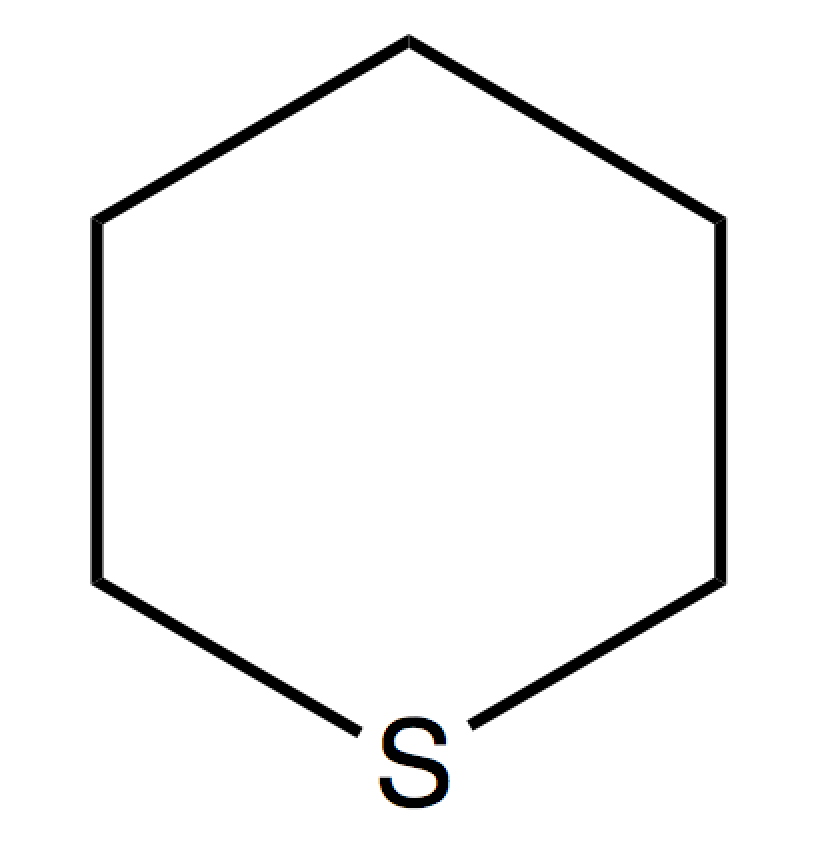
\includegraphics[scale=0.08]{../image/sulfure-cycle} & Sulfures cycliques \\
			RSSR' & Disulfures \\
			 
\includegraphics[scale=0.08]{../image/thiophene} & Thiophène \\
			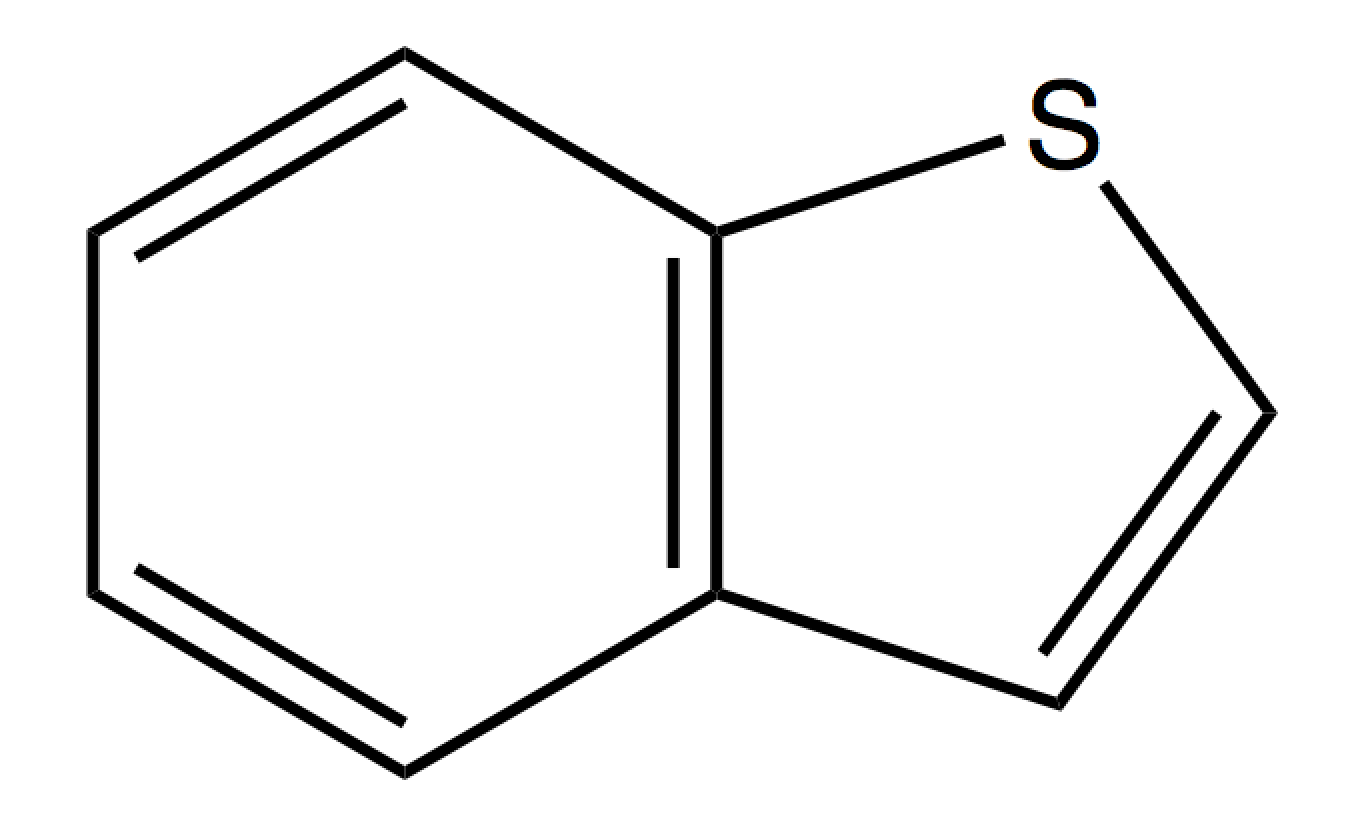
\includegraphics[scale=0.08]{../image/benzothiophene} & Benzothiophène \\
			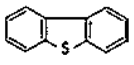
\includegraphics[scale=0.08]{../image/dibenzothiophene} & Dibenzothiophène \\
			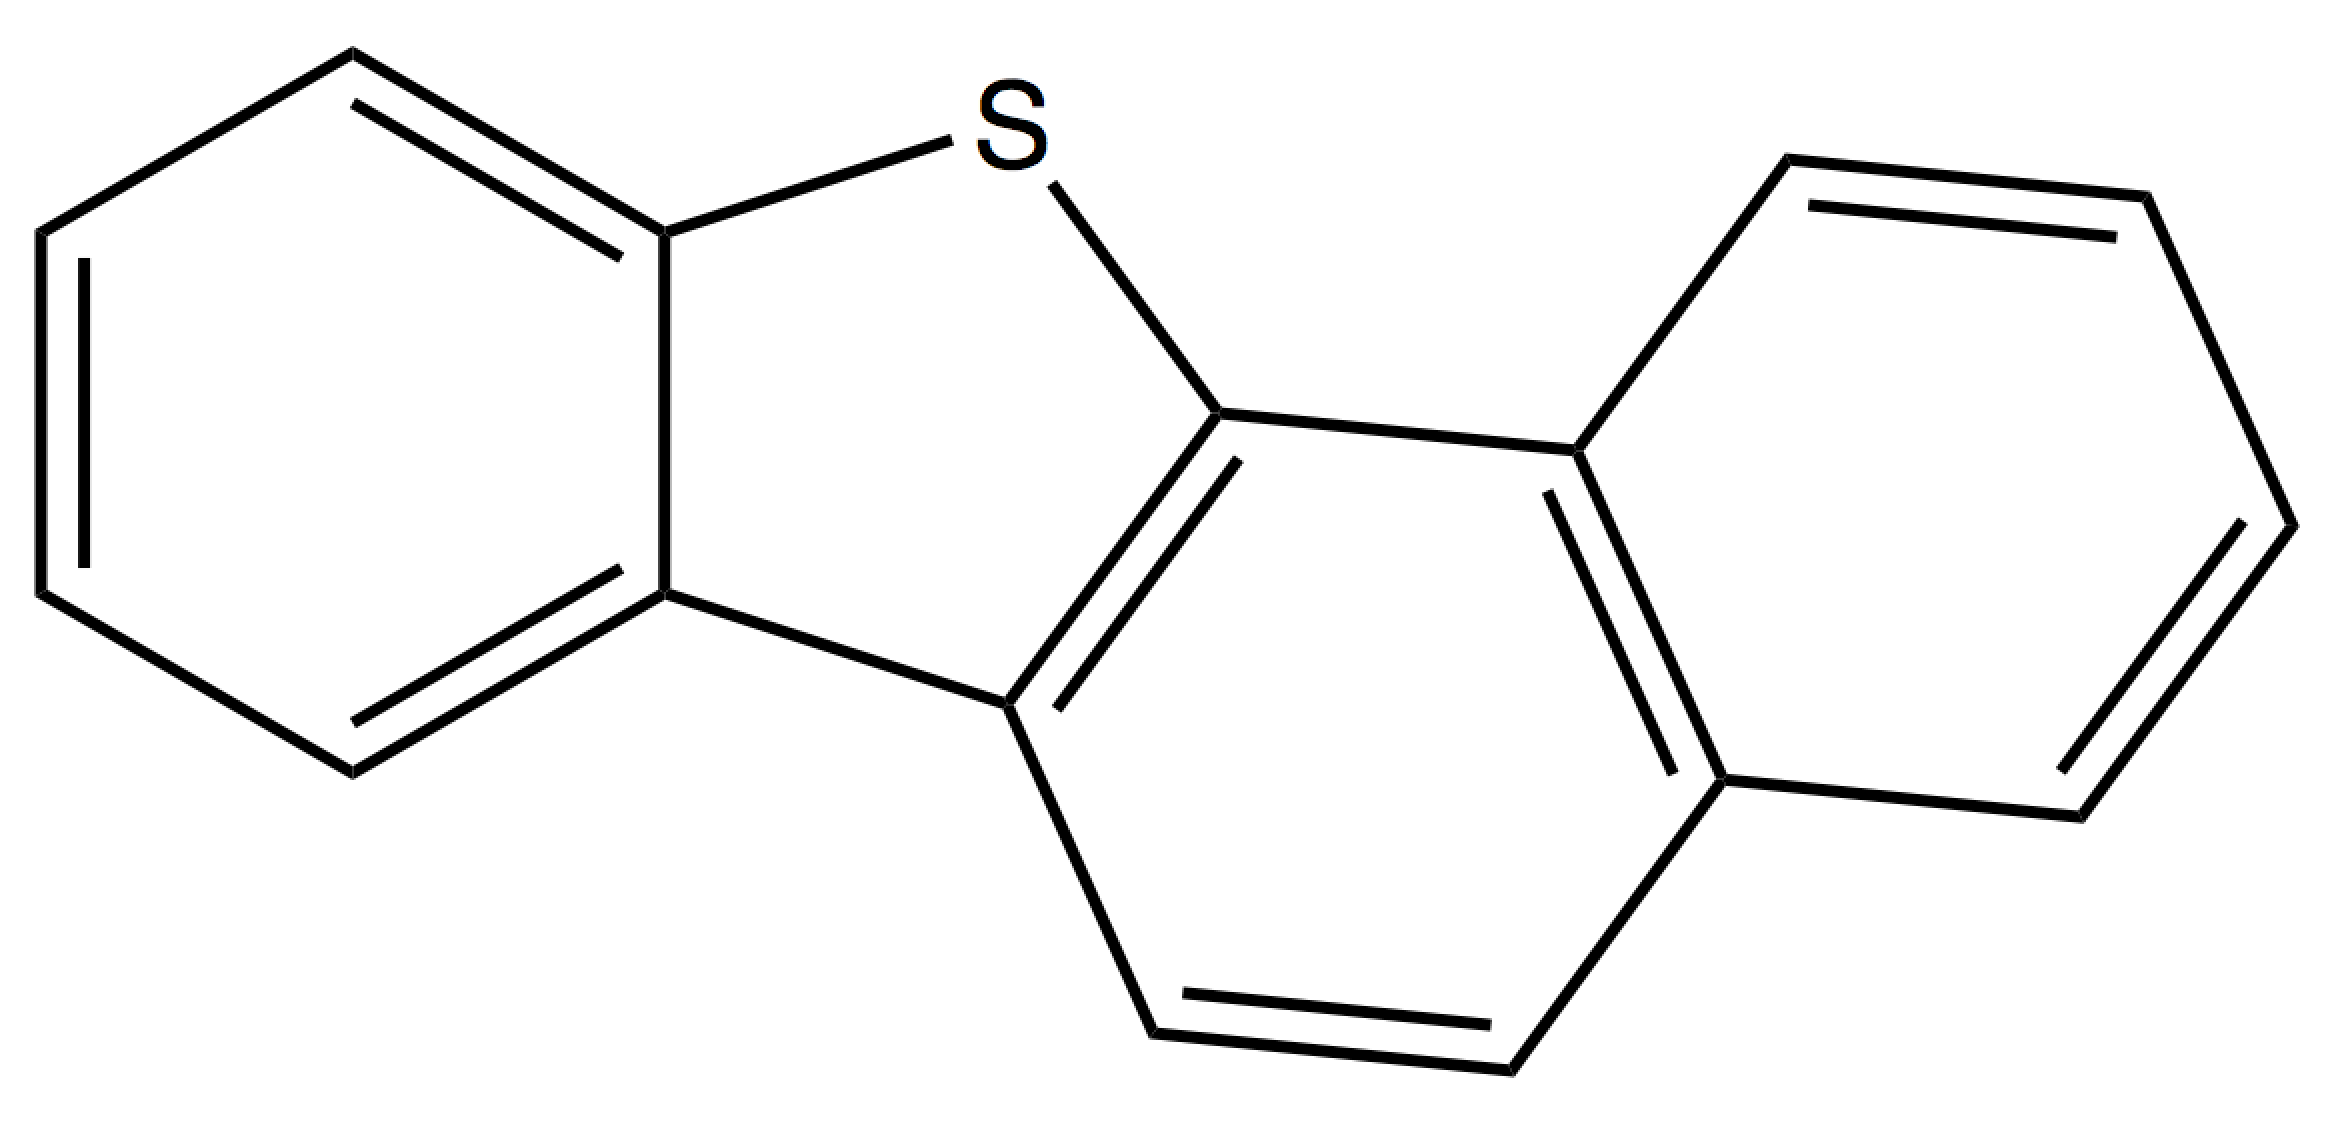
\includegraphics[scale=0.08]{../image/naphto1} & Naphtobenzothiophènes \\
			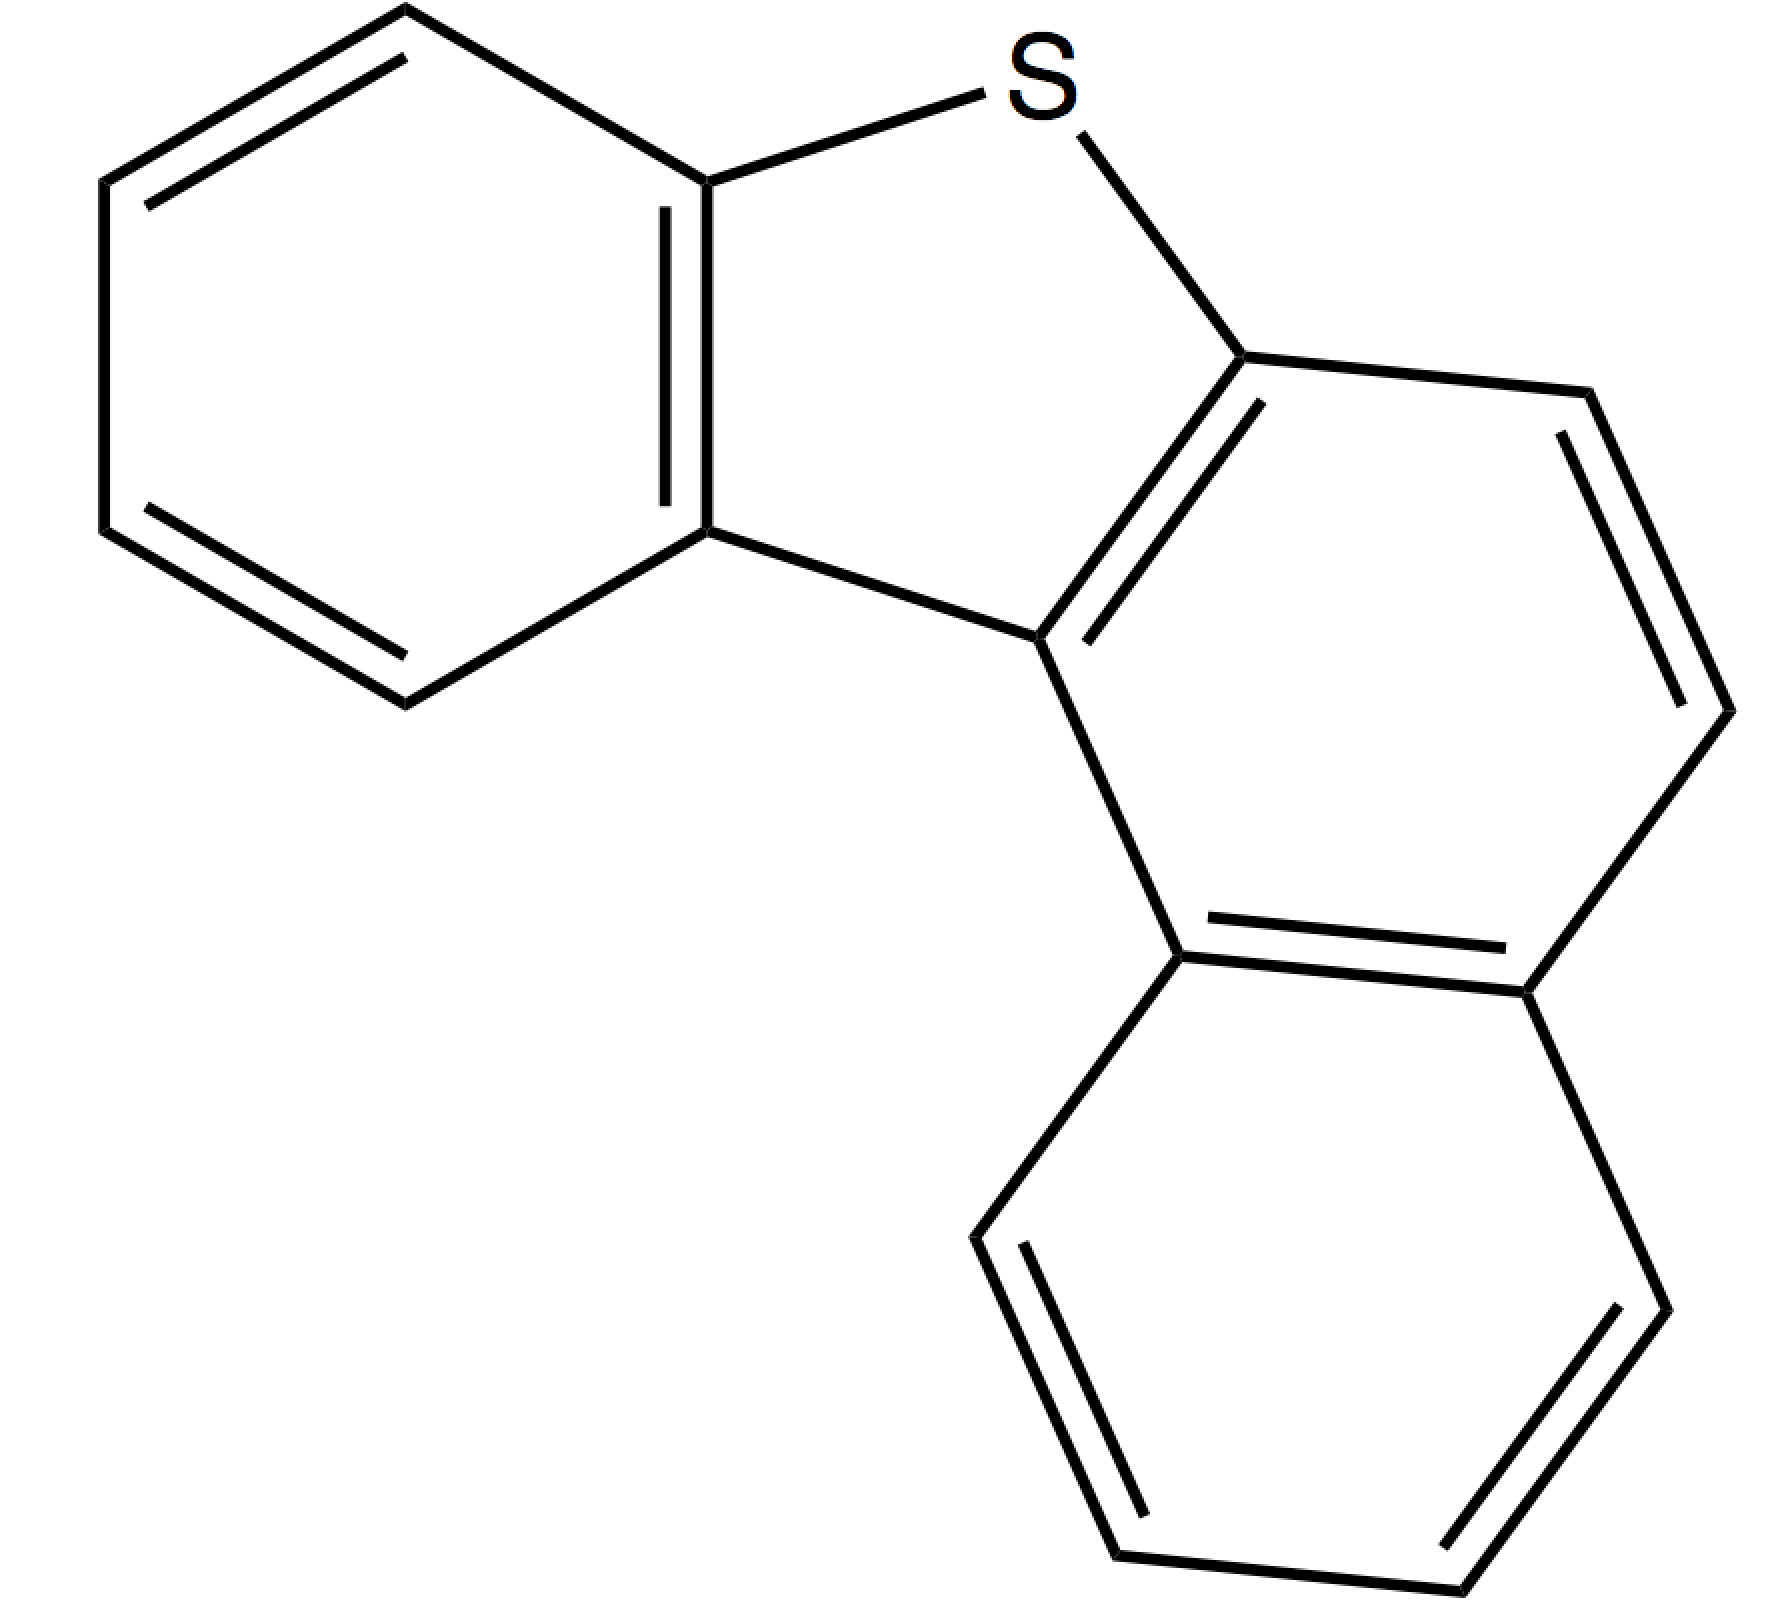
\includegraphics[scale=0.08]{../image/naphto2} & \\
			\hline 
		\end{tabular}
	\end{center}
	\caption{Famille de composés soufrés caractérisés au sein du pétrole brut}
	\label{tab:soufre}
\end{table}


Thiols, sulfures, sulfoxydes et disulfides peuvent être classés plus précisément suivant leur nature cyclique ou acyclique, soit suivant l'organisation du squelette carboné (alkyle, aryle ou alkyl-aryle). Les dérivés thiophéniques, quant à eux, sont des structures polyaromatiques condensées autour d'un noyau thiophène (benzo, dibenzo, naphtobenzo-thiophènes, etc.). Au sein des fractions lourdes, la majorité des espèces soufrées sont des dérivés thiophéniques (cf. tableau \ref{tab:soufre-ex}), suivi par des dérivés sulfures (cycliques et acycliques). Enfin, des espèces de type sulfoxydes ont été mises en évidence, dans des proportions très variables, leur teneur variant entre 0.3\% et 10.3\% \cite{merdrignac2007physicochemical, speight2004petroleum}.

\begin{table}[h!]
	\begin{center}
		\begin{tabular}{rl}
			\hline
			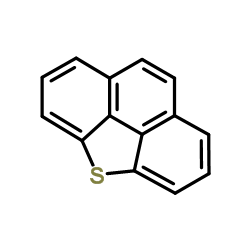
\includegraphics[scale=0.4]{../image/phenanthro-thiophene} & Phénanthro-thiophènes \\
			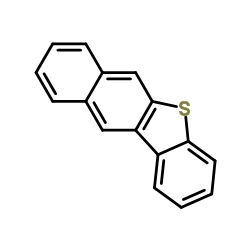
\includegraphics[scale=0.4]{../image/benzo-naphto-thiophene} & Benzonaphto-thiophènes \\
			\hline 
		\end{tabular}
	\end{center}
	\caption{Exemples de dérivés thiophéniques courants identifiés au sein des fractions lourdes : phénanthro-thiophènes et benzonaphto-thiophènes}
	\label{tab:soufre-ex}
\end{table}


\paragraph{Azote}
En dépit des faibles proportions dans lesquelles il est présent, les dérivés de l'azote sont particulièrement étudiés, puisqu'à l'origine de la destruction des catalyseurs employés lors du craquage. Comme leurs analogues soufrés, les composés azotés se retrouvent en majeure partie au sein des fractions lourdes et des résidus de distillation du pétrole. \\
On distingue communément deux classes de composés azotés, à savoir les dérivés dits \og \textit{basiques} \fg, qui regroupent les homologues de la pyridine, et les dérivés dits \og \textit{neutres} \fg, qui rassemblent des systèmes de type pyrrole, indole et carbazole.  
En règle générale, environ un tiers des composés azotés sont des dérivés "basiques", la part restante revenant donc aux composés dits "neutres", bien que ces proportions puissent varier sensiblement en fonction des paramètres géochimiques de provenance du pétrole. \\
Comme indiqué dans le tableau \ref{tab:azote}, les structures "basiques" identifiées sont des analogues de la pyridine, tels que la quinoléine ou l'iso-quinoléine, comprenant entre deux et quatre cycles aromatiques condensés avec différents degrés d'alkylation ; des benzo- et dibenzoquinoléines, tétrahydroquinoléines, ainsi que des azapyrènes, ont par exemple pu être caractérisés, qui forment autant de systèmes à haut encombrement stérique. \\

\begin{table}[h!]
	\begin{center}
		\begin{tabular}{rl}
			\hline
			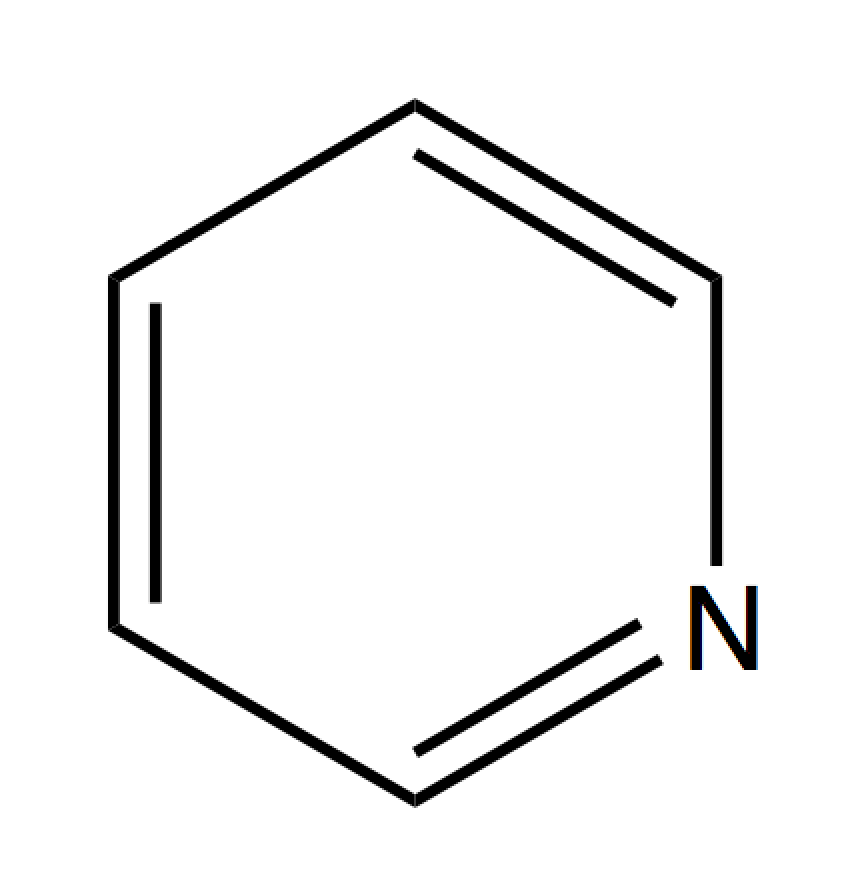
\includegraphics[scale=0.08]{../image/pyridine} & Pyridine \\
			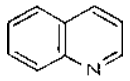
\includegraphics[scale=0.08]{../image/quinoline} & Quinoline \\
			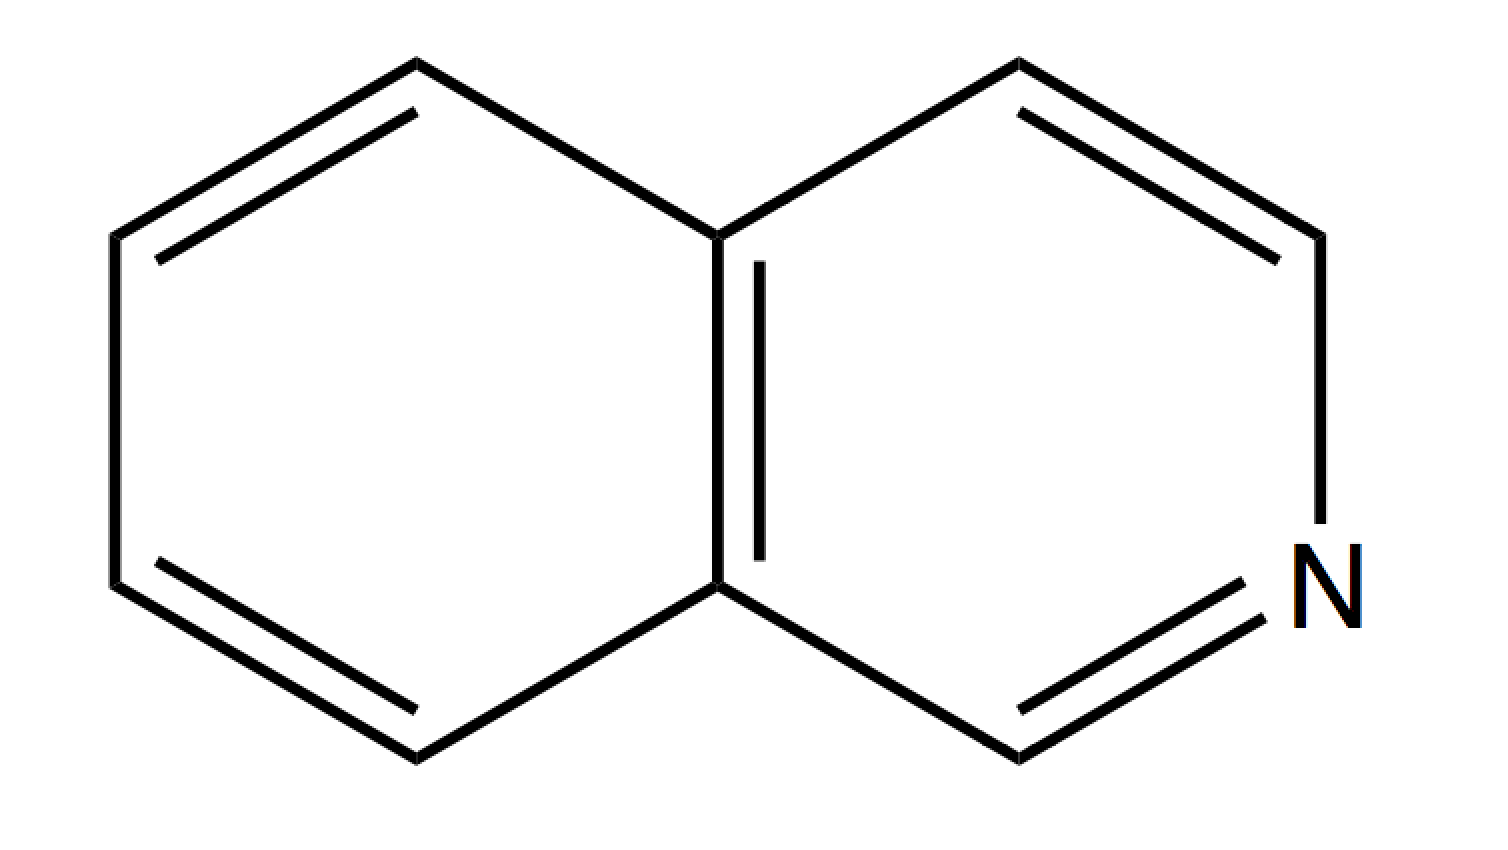
\includegraphics[scale=0.08]{../image/isoquinoline} & Isoquinoline \\
			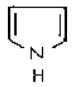
\includegraphics[scale=0.08]{../image/pyrrole} & Pyrrole \\
			\includegraphics[scale=0.08]{../image/Indole} & Indole \\
			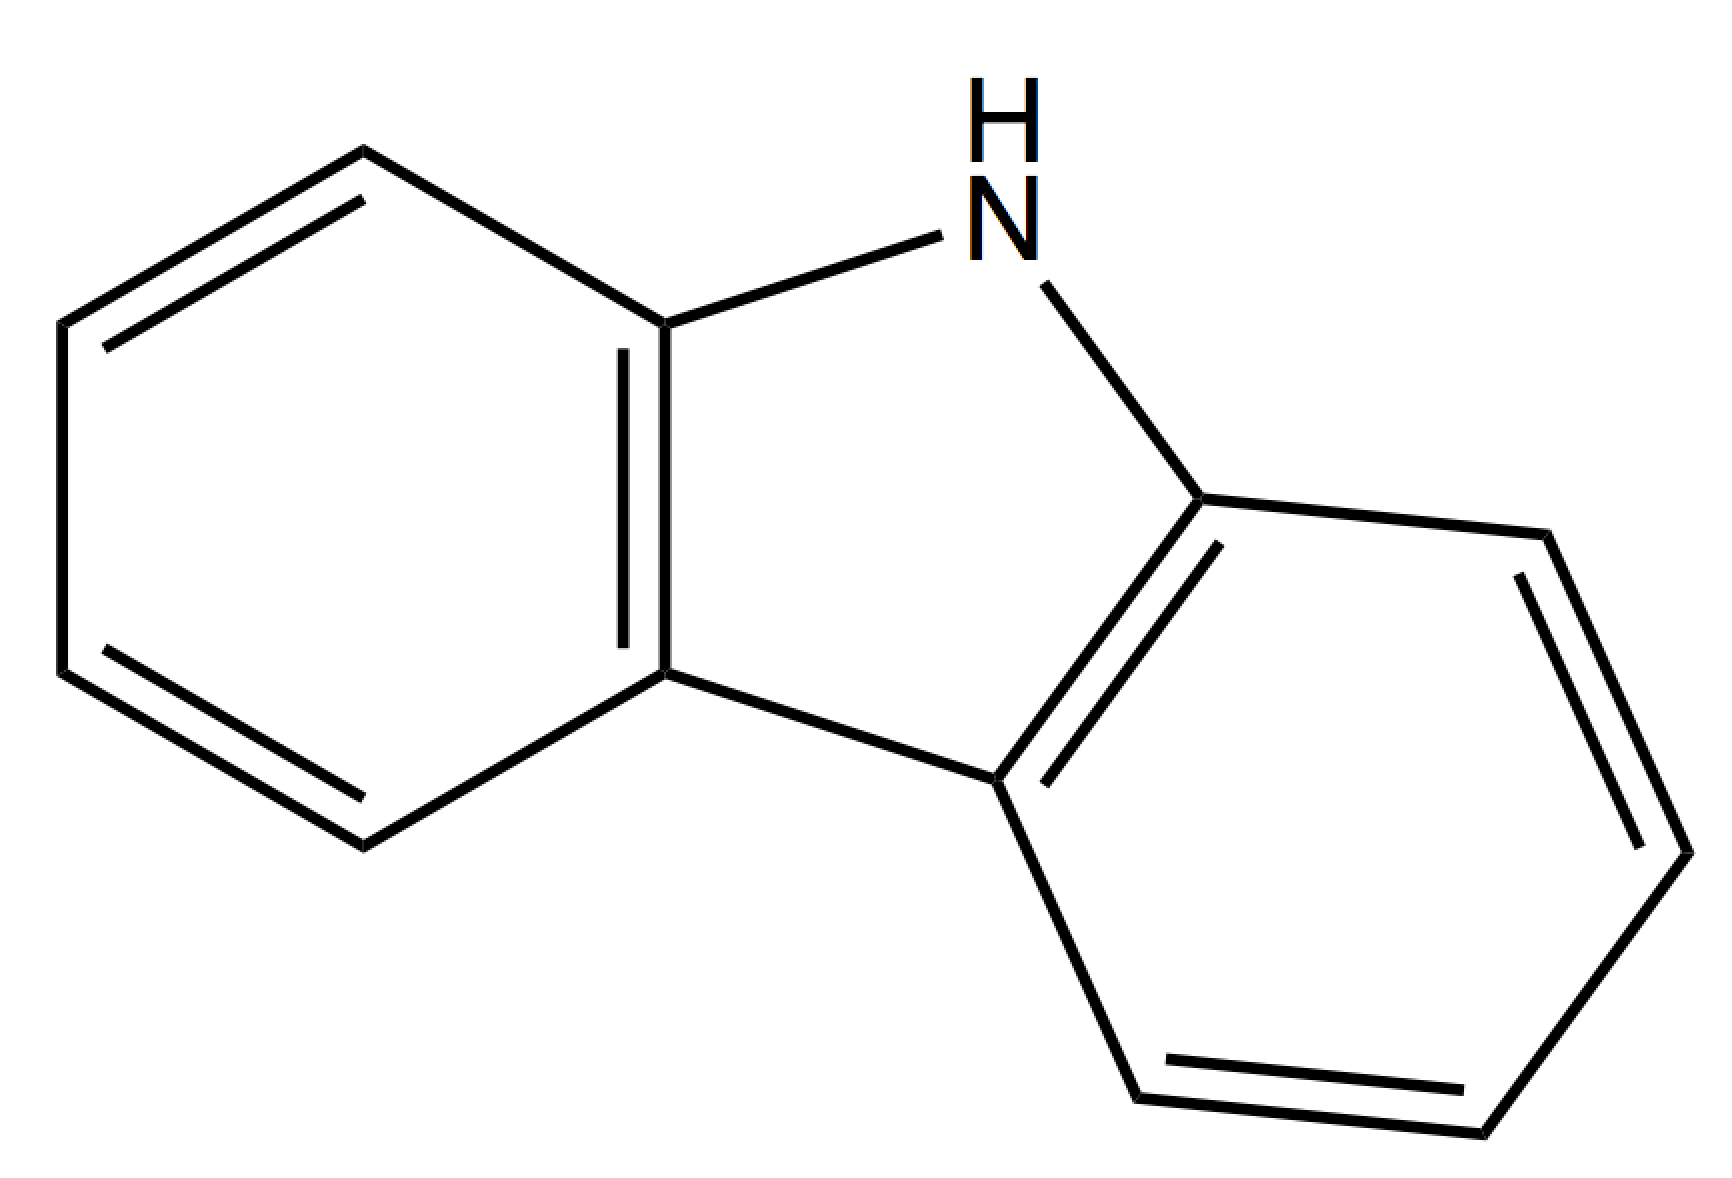
\includegraphics[scale=0.08]{../image/carbazole} & Carbazole \\
			\hline 
		\end{tabular}
	\end{center}
	\caption{Famille de composés azotés caractérisés au sein du pétrole brut}
	\label{tab:azote}
\end{table}


Les structures "neutres", majoritaires, sont essentiellement représentées par les dérivés carbazolés (benzo-carbazoles, dibenzo-carbazole, etc.). C'est également au sein de cette classe de composés que l'on trouve les porphyrines qui, bien que présentes en proportions plus anecdotiques, possèdent une stabilité remarquable. La brique élémentaire de ces systèmes de grande taille est la molécule de pyrrole, et la plus simple des porphyrines est constituée par l'assemblage de quatre molécules de pyrrole [figure porphine !!!], reliées par des ponts méthylène =CH--. Le large système de résonance ainsi formé augmente considérablement la stabilité des structures ainsi formées. Par ailleurs, les porphyrines ont tendance à former des complexes métalliques avec les ions nickel et vanadium présents au sein du pétrole, par substitution des deux atomes d'hydrogène liés aux atomes d'azote de la structure porphyrinique. La proportion de ces structures au sein du pétrole dépend une nouvelle fois de l'origine géochimique de ce dernier, et un nombre croissant d'études s'intéresse à la part de métaux présents dans les huiles brutes. On estime aujourd'hui que ces complexes porphyrine-métaux représentent entre 0.6 et 3.3\% des fractions lourdes extraites\cite{merdrignac2007physicochemical, speight2004petroleum}.

\paragraph{Oxygène}
Au sein des fractions lourdes qui nous intéressent, la teneur en composés oxygénés varie entre 0.3 et 4.9\% \cite{speight2004petroleum}. Ces composés oxygénés figurent parmi les premières espèces caractérisées du pétrole. Les premiers travaux reportant la présence d'espèces acides au sein du pétrole remontent à 1874, et il faudra attendre quelques années de plus avant que celles-ci ne soient formellement identifiées comme étant des acides carboxyliques. Avec les dérivés du phénol, les acides carboxyliques représentent la majorité des espèces oxygénées constituant le pétrole, que l'on retrouve aussi bien dans les fractions lourdes qu'au sein de fractions plus légères. L'ensemble des études réalisées sur le sujet tend à établir que la structure de ces acides carboxyliques correspond à la structure de l'hydrocarbure prévalent. En d'autres termes, la structure de l'acide dépend du nombre d'atomes de carbone que compte le squelette carboné de l'hydrocarbure. Ainsi, lorsque l'acide comporte moins de huit atomes de carbone, ce qui correspond à un hydrocarbure de type paraffinique comme évoqué ci-avant, sa structure sera de type aliphatique. Suivant cette logique, des acides comportant un cycle commencent à apparaître à partir de six atomes de carbone et ces structures monocycliques prédominent jusqu'à quatorze atomes de carbone environ. \\
Une caractérisation plus fine des groupements carboxyles en présence révèle également la coexistence d'esters, de cétones, d'amides, d'anhydrides, d'éthers et de sulfoxydes. Néanmoins, à la différence des acides carboxyliques, plus aisés à caractériser puisque présent tant dans les fractions lourdes que dans les fractions légères, ces composés oxygénés se retrouvent majoritairement dans les fractions lourdes et leurs structures sont de fait plus complexes à identifier. Il est par ailleurs à noter que certains de ces composés sont supposés provenir de réactions entre les résidus de distillation et l'oxygène soufflé, qui intervient notamment dans les procédés de production de l'asphalte. De fait, il est difficile de conclure quant au fait que toutes ces espèces sont ou non des constituants du pétrole brut. 


\subsubsection{Débat autour du poids moléculaire des asphaltènes}

Un rapide passage en revue de la bibliographie des asphaltènes révèle tout le débat autour de leur poids moléculaire. En effet, la distribution, en termes de poids moléculaire, varie entre 400 et 1500 Da pour les fractions de faible poids moléculaire, et peut atteindre $10^{6}$ Da pour les fractions de haut poids moléculaire \cite{mullins2008contrasting}. Le phénomène d'agrégation des asphaltènes est une des raisons avancées pour justifier qu'à l'heure actuelle aucune méthode n'ait permis de déterminer avec précision le véritable poids moléculaire de ces espèces. De nombreux procédés ont été employés pour tenter de résoudre ce problème, mais ceux-ci conduisent à des résultats ambigüs, qu'il serait hasardeux de généraliser. À titre d'exemple, des mesures par osméométrie à tension de vapeur font apparaître des résultats fortement dépendants du type de solvant employé ; en présence d'un solvant apolaire tel que le toluène, les résultats apparaissent surestimés, au contraire de l'utilisation d'un solvant polaire tel que la pyridine ou le nitrobenzène. 
%S'agissant d'autres méthodes d'analyse, Groenzin et Mullins\cite{groenzin2000molecular} parviennent, par spectroscopie de fluorescence résolue en temps, à un poids moléculaire moyen de 750 Da environ, pour une distribution de 500 à 1000 Da, là où Pinkston et col.\cite{pinkston2009analysis} rapportent une distribution de 350 à 1050 Da pour une étude par spectrométrie de masse de résonance cyclotronique ionique à transformée de Fourier (FT-ICR). Ces derniers supposent l'existence de fragments de plus bas poids moléculaires, non détectés même à haute énergie électronique du fait de la stabilisation des intermédiaire obtenus par les chaînes alkyles des asphaltènes. 

%Merdrignac et col.\cite{merdrignac2006evolution} rapportent l'évolution du poids moléculaire des asphaltènes et comparer les changements causés par le procédé d'hydroconvertion. 


%\subsubsection{Une inconnue : la structure des asphaltènes}

\section{État des lieux des connaissances sur les systèmes asphalténiques}

La description de la structure des asphaltènes repose à l'heure actuelle sur deux modèles construits sur la base des résultats de diverses caractérisations expérimentales.  
Le premier modèle, baptisé modèle \og continental \fg, représente les asphaltènes comme de larges cœurs constitués de quatre à dix cycles aromatiques condensés, ramifiés par des chaînes alkyles courtes \cite{groenzin2000molecular} (cf. figure \ref{figZ1}). Ce modèle a été proposé par Zhao \textit{et al.} \cite{zhao2001molecular} après caractérisation des asphaltènes obtenus par fractionnement avec du pentane supercritique, puis remployé par Rogel et Carbognani \cite{rogel2003density} dans leur travail sur des asphaltènes stables et instables extraits de pétrole provenant du Vénézuela. 
Ce type de représentations est corrélé par des analyses en spectroscopie RMN, diffraction des rayons X et spectroscopie de fluorescence résolue en temps (TRDF). 



\begin{figure}[h!]
	\centering
	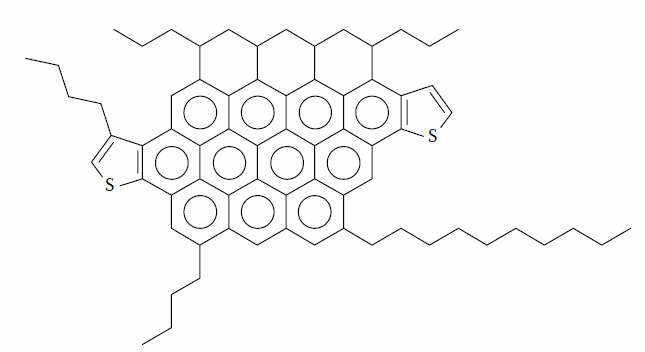
\includegraphics[height=5cm]{../image/Zhao}
	\caption[Structure moyenne du modèle continental des asphaltènes]{Structure moyenne du modèle continental des asphaltènes (Zhao et col. \cite{zhao2001molecular})}
	\label{figZ1}
\end{figure}


Le modèle "archipel" présente quant à lui ces systèmes comme un ensemble de régions à caractère aromatique, constituées de deux à trois cycles condensés, reliées par des chaînes carbonées. Ce modèle s'appuie sur des analyses par pyrolyse, oxydation, dégradation thermique et dispersion angulaire neutronique, telles que rapportées par Gawrys \textit{et al.} \cite{gawrys2003role}. Sheremata \textit{et al.}\cite{sheremata2004quantitative} ont notamment employé ce modèle pour la description des asphaltènes, comme le présente la figure reproduite ci-après (figure \ref{fig2}). 

\begin{figure}[h!]
	\centering
	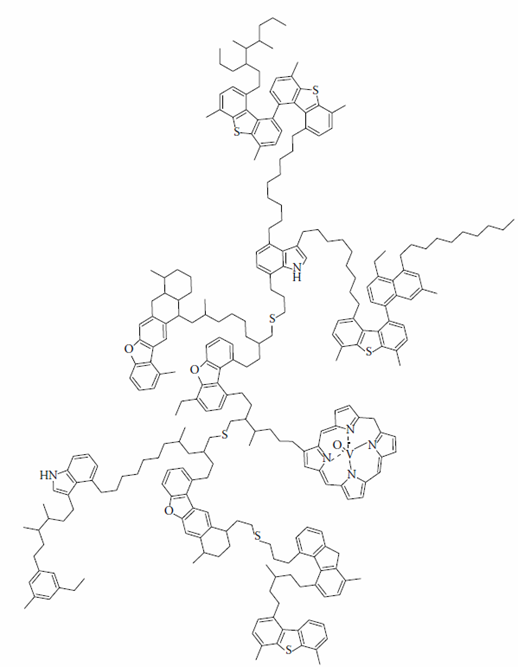
\includegraphics[height=8cm]{../image/Sher}
	\caption[Molecule d'asphaltènes type archipel]{Représentation d'asphaltènes à l'aide du modèle archipel, proposé par Sheremata \textit{et al.}\cite{sheremata2004quantitative}}
	\label{fig2}
\end{figure}

Ces deux modèles, basés sur des structures moléculaires bien distinctes, conduisent néanmoins à des propriétés physico-chimiques différentes. La description des agrégats d'asphaltènes ainsi que leur solubilité dans le pétrole brut seront nettement impactées par l'emploi de l'une ou l'autre de ces représentations. Du fait de la planéité induite par la présence d'un grand nombre de cycles aromatiques condensés, la représentation d'un agrégat d'asphaltènes dans le cadre du modèle continental conduit à un empilement de plans. À l'inverse, les chaînes alkyles du modèle archipel confèrent une toute autre géométrie à ces systèmes : les asphaltènes peuvent se courber par le biais d'interactions intermoléculaires pour former des macro-agrégats globulaires susceptibles de piéger les molécules de solvant. \bigskip

Le paragraphe qui suit se veut résumer les nombreuses analyses expérimentales menées sur ces systèmes, analyses qui ont dans un premier temps permis l'émergence des deux modèles que nous venons d'évoquer, avant de travailler à les confirmer ou les infirmer. 

\subsection{Revue des données expérimentales}

\subsubsection{Analyses par spectroscopie RMN}

La spectroscopie de résonance magnétique nucléaire est couramment employée pour l'analyse structurale et la caractérisation de matériaux et de substances organiques. 
%Elle est fondée sur les propriétés magnétiques de certains noyaux atomiques.Les noyaux les plus étudiés, dans le cadre de la chimie organique sont l'hydrogène $^{1}H$ et le carbone $^{13}C$. 
Cette technique représente donc une méthode d'analyse de choix pour l'étude des asphaltènes et a, à ce titre, permis d'acquérir les premiers résultats visant à résoudre leur composition chimique. Dès 1982, les travaux de Murphy \textit{et al.} \cite{murphy1982determination} révèlent que la structure primaire des asphaltènes se compose de multiples cycles aromatiques condensés (l'indice de condensation relevé sur ces systèmes étant de 3 au moins) ainsi que d'une grande variété de chaînes aliphatiques, longues et ramifiées. Par la suite, les travaux de Yen \textit{et al.} en RMN $^{1}H$ ont donné une première idée de la proportion d'hydrocarbures saturés en regard de la fraction d'hydrocarbures aromatiques au sein de molécules d'asphaltènes  \cite{yen1984study}. Enfin, plus récemment, Durand \textit{et al.} ont employé les résultats de leurs analyses par RMN $^{13}C$ pour évaluer les indices de substitution et de condensation d'échantillons d'asphaltènes de différentes origines \cite{durand2010effect}. Leur étude tend à démontrer qu'au sein d'agrégats d'asphaltènes cohabitent les deux modèles structuraux évoqués ci-avant, à savoir le modèle continental et le modèle archipel. 


\subsubsection{Analyses par diffraction des rayons X}  

Une étude du caractère aromatique et des paramètres cristallins des asphaltènes, des résines et des gilsonites issus du pétrole a été présentée par Yen \textit{et al.} sur la base d'analyses en diffraction des rayons X \cite{yen1961investigation}. Leurs résultats, confortés par les travaux réalisés par Shirokoff \textit{et al.} sur quatre échantillons d'asphaltènes issus d'huiles brutes provenant d'Arabie Saoudite \cite{shirokoff1997characterization}, représentent les asphaltènes comme des feuillets de cycles aromatiques condensés portant des ramifications de natures naphténiques et aromatiques.
Toutefois, Altget et Boduszynky rappellent judicieusement dans leur étude \cite{altgeltcomposition} qu'il convient de prendre avec précaution les résultats provenant d'analyses de diffraction, lorsque les données géométriques fournies par l'analyse servent de base pour construire un modèle structural du système étudié. Leurs travaux semblent en outre indiquer que la détermination du caractère aromatique des asphaltènes est, par ce biais, inappropriée sinon arbitraire. 



\subsubsection{Analyses par spectroscopie de fluorescence résolue en temps} 

Cette méthode d'analyse a été employée à plusieurs reprises pour tenter d'élucider plus précisément la taille et la structure de molécules d'asphaltènes faiblement agrégées.  
Les premiers travaux en ce sens, réalisés par Groenzin et Mullins  \cite{groenzin1999asphaltene}, tendent à montrer que les molécules d'asphaltènes ne seraient constituées que d'un seul groupe chromophore. En effet, le faible poids moléculaire obtenu pour ces systèmes, comme la coloration des molécules, sont autant d'éléments recueillis incompatibles avec la représentation des asphaltènes sous forme de larges structures pseudo-polymériques constitués de deux ou trois cycles aromatiques reliés entre eux par de longues chaînes aliphatiques. En définitive, ces premières analyses par spectrométrie de fluorescence semblent conforter la représentation des asphaltènes par le modèle continental. \\
Par la suite, Souza \textit{et al.} ont rapporté l'agrégation persistante des asphaltènes à la faible concentration de 0.8 g/L, soit sous le seuil de concentration critique de nanoagrégation \cite{souza2009study}. Leurs travaux corroborent par ailleurs les résultats de Groenzin \textit{et al.}\cite{groenzin1999asphaltene} quant à la structure de type \og continental \fg{} des molécules d'asphaltènes, en cela qu'ils concluent à une structure primaire constituée d'un anneau polyaromatique de quatre cycles ou plus. 




\subsubsection{Analyses par spectroscopie infrarouge}

La caractérisation d'un système chimique en termes de composition passe nécessairement par des analyses en spectroscopie infrarouge, laquelle permet l'identification des groupements fonctionnels. Toutefois, dans le cadre de l'étude des fractions lourdes du pétrole, la diversité chimique et la taille des espèces présentes rendent complexe l'utilisation de la spectroscopie IR. C'est ce que soulignent Yuan \textit{et al.}, qui relèvent l'existence d'un faible nombre d'analyses employant l'infrarouge moyen pour la caractérisation physique et chimique des huiles lourdes \cite{hongfu2006determination}. 
Parmi les travaux notables, l'étude couplée en spectroscopies IR et UV-sisible menée par El-Bassoussi \textit{et al.}\cite{el2010characterization} sur deux échantillons d'asphaltènes provenant d'Egypte a permis de classifier les espèces présentes en mono, di et polyaromatiques. En accord avec les deux modèles de représentation des asphaltènes, les espèces prédominantes sont les espèces di ou polyaromatiques. En 2007, Rodrigues Coelho \textit{et al.} \cite{coelho2007characterization} démontrent l'existence d'une corrélation linéaire entre les intensités des bandes infrarouges symétriques et antisymétriques associées aux atomes d'hydrogène aromatiques de type arènes méthyl-substitués dans les régions 2900-3100 $cm^{-1}$ et 700-900 $cm^{-1}$. Enfin, Laxalde \textit{et al.} \cite{laxalde2014combining} rapportent une interprétation, toutefois ajustée sur les structures modèles des asphaltènes, en repérant les vibrations de stretching des liaisons C-H (hors du plan) et C=C.

\bigskip

\subsubsection{Conclusion : les asphaltènes, une coexistence de structures moléculaires ?}

La compilation de l'ensemble de ces résultats expérimentaux tend à suggérer que les deux modèles structuraux des asphaltènes peuvent coexister au sein des fractions lourdes. Cette idée est appuyée par les résultats d'Acevedo \textit{et al.} \cite{acevedo2004structural, gutierrez2001fractionation} qui ont montré que les asphaltènes pouvaient se diviser en deux fractions : une fraction insoluble dans le toluène, baptisée A1, qui serait rigide et plane, conformément au modèle continental, et une fraction soluble dans le toluène grace à de nombreuses interactions intermoléculaires, baptisée A2 et qui correspondrait au modèle archipel. Sur la base de ces éléments, Acevedo et son équipe ont mis en place une nouvelle représentation des agrégats d'asphaltènes. Le système colloïdal consisterait en une fraction d'asphaltènes A1, entourés par une couche d'asphaltènes A2, ces derniers aidant à la solubilisation de l'ensemble. \\
En définitive, une revue bibliographique des analyses expérimentales menées à ce jour sur les asphaltènes montre qu'aucun modèle structural définitif valide n'a encore émergé pour ce type de systèmes. De nombreux travaux cherchent encore à clarifier l'architecture moléculaire des asphaltènes, à deux échelles distinctes. En premier lieu, l'étude de la microstructure correspond à des systèmes de poids moléculaires variant entre 500 et 10 000 Da, soit à des nano-agrégats d'asphaltènes. En second lieu, les travaux sur la macrostructure de ces entités correspondent à l'étude d'assemblages de ces nano-agrégats d'asphaltènes et sont intimement liés au milieu. 



\subsection{La modélisation, outil indispensable dans l'élucidation des structures asphalténiques}

\subsubsection{Des nombreux intérêts de la modélisation des asphaltènes}

La chimie computationnelle a révolutionné notre façon d'appréhender la structure et la réactivité des molécules, de sorte que la simulation est désormais une des clés de voûte de l'avancée scientifique. \\
Comme nous l'avons souligné dans le paragraphe précédent, la nature et la complexité des asphaltènes rendent impossible leur caractérisation exhaustive par le seul biais de données expérimentales. Dans ce cadre, l'intérêt des simulations est incontestable et nombreux sont les travaux qui se sont déjà penchés sur la configuration moléculaire, les interactions intermoléculaires, la stabilité ou les phénomènes d'agrégation de ces systèmes.  
Concernant ce dernier point, la modélisation moléculaire a permis de justifier que l'agrégation des asphaltènes représentait la conformation la plus stable, sur la base d'une double approche structurale et thermodynamique révélant les interactions avec les résines, présentes au sein des fractions lourdes, et les solvants \cite{murgich1996molecular}. Selon ces travaux, l'interaction responsable de la formation comme de la stabilité des micelles formés d'asphaltènes et de résines serait la force d'attraction qui s'exerce entre les plans aromatiques. 
D'autres études théoriques se fondent sur les modèles structuraux proposés pour les asphaltènes. Les orbitales moléculaires de dimères d'asphaltènes, envisagés successivement par les modèles continental et archipel, ont été étudiés dans une approche semi-empirique ZINDO après optimisation des structures en DFT (théorie de la fonctionnelle de la densité). Du point de vue de la stabilité, la configuration continentale, représentée dans les simulations par des dimères empilés pour symboliser les plans d'asphaltènes propres à ce modèle, s'avère globalement plus stable que la configuration archipel \cite{alvarez2013island}. 


\subsubsection{Construction de la structure moléculaire des asphaltènes}

La construction d'un modèle moléculaire utilisable en simulation se fait sur la base des données expérimentales recueillies, suivant deux méthodes principales. \\
La première méthode repose sur une corrélation des résultats empiriques utilisés pour déduire des informations structurales. Dans le cas des asphaltènes, l'existence de nombreux cycles aromatiques et l'ensemble des données obtenues concernant la longueur des chaînes aliphatiques ont permis à Takanohashi \textit{et al.} d'étudier trois structures distinctes d'asphaltènes générées par la méthode de Sato par le biais de simulation en dynamique moléculaire \cite{takanohashi2004structural}. \\
La seconde méthode consiste à identifier des caractéristiques structurales propres au système, ainsi que sa composition moléculaire, en suivant un processus stochastique. Le modèle structural se construit alors par addition des données expérimentales et/ou par recoupement de ces résultats avec une base de données existantes. Cette méthode a été poursuivie aussi bien par Elyashberg \textit{et al.} \cite{elyashberg2008computer}, qui ont développé un algorithme permettant la construction d'une structure sur la base de données RMN, que par Todeschini \textit{et al.} \cite{todeschini1995weighted} qui ont quant à eux employé des propriétés physiques telles que l'hydrophobie, le point de fusion et le point d'ébullition. 
La construction d'un modèle moléculaire des asphaltènes peut en dernier lieu se faire initialement de façon plus intuitive, les informations expérimentales servant ensuite à optimiser le modèle de départ \cite{faulon1996stochastic}, \cite{al2012systematic}, \cite{de2012monte}. 



\renewcommand{\bibname}{Références bibliographiques}
\bibliography{biblio}
\bibliographystyle{unsrt}

\end{document}